% This is samplepaper.tex, a sample chapter demonstrating the
% LLNCS macro package for Springer Computer Science proceedings;
% Version 2.20 of 2017/10/04
%
\documentclass[runningheads]{llncs}
%
\usepackage{graphicx}
\usepackage{amssymb}
\usepackage{algorithmicx}
\usepackage{algorithm2e}
\usepackage[utf8]{inputenc}
\usepackage{subfig}
% Used for displaying a sample figure. If possible, figure files should
% be included in EPS format.
%
% If you use the hyperref package, please uncomment the following line
% to display URLs in blue roman font according to Springer's eBook style:
% \renewcommand\UrlFont{\color{blue}\rmfamily}

\begin{document}
%
\title{Interactive Visualization of Large Bipartite Networks Assisted by Multilevel Strategies\thanks{Supported by FAPESP, project 2017/05838-3}}
%
\titlerunning{Multilevel Visualization of Bipartite Networks}
% If the paper title is too long for the running head, you can set
% an abbreviated paper title here
%
\author{Renato Fabbri\orcidID{0000-0002-9699-629X} \and
Alan Valejo \and
Maria Cristina Ferreira de Oliveira\orcidID{0000-0002-4729-5104}}
%
\authorrunning{R. Fabbri et al.}
% First names are abbreviated in the running head.
% If there are more than two authors, 'et al.' is used.
%
\institute{University of São Paulo, São Carlos SP, BR\\
\email{renato.fabbri@gmail.com},
\email{alanvalejo@gmail.com},
\email{cristina@icmc.usp.br}\\
\url{http://conteudo.icmc.usp.br/pessoas/cristina/}}
%
\maketitle
%
\begin{abstract}
% The abstract should briefly summarize the contents of the paper in
% 150--250 words.
  It is a well established fact that bipartite, or two-layer, networks are pervasive
  in modeling real-world phenomena and that they play fundamental roles in
  graph theory.
  Multilevel strategies have been developed for optimization tasks,
  and for the visualization of simple (``unipartite'') networks,
  but their employment for visualizing bipartite networks were not found by the authors.
  In this work, we present advances in the use of multilevel strategies for the
  visualization of bipartite networks,
  allowing for interactive and intuitive navigation of such structures and visual mappings of large datasets.
  More specifically, we developed a web-based visualization interface in which
  a parametrizable simplification of
  bipartite networks are obtained through the application of coarsening algorithms.
  The resulting networks are then presented to the user,
  providing a genuine route for the ``overview first - focus on demand''
  process on the analysis of the underlying data, in which the analyst
  selects supervertices or whole network sectors for more detailed observation,
  i.e. performs requests for the interface to display 
  specific structures in less simplified settings.
  The application allows not only the visualization of large networks,
  but also for an on-demand navigation of the multilevel structure,
  and is useful for the further development multilevel strategies themselves
  e.g. by the specification of vertices to guide the coarsening processes and
  the examination of the resulting multilevel hierarchy.

\keywords{Network visualization \and Bipartite networks \and Multilevel strategies \and Big data \and Complex networks \and Data visualization.}
\end{abstract}
%
\section{Introduction}
The visualization of large-scale networks poses challenges both in terms of computational costs
and of effective presentation of the information to the user~\cite{tang,staudt}.
These issues may be aggravated in the case of bipartite networks,
due to their sparsity and topological complexities.
Bipartite networks are comprised of two partitions of nodes,
called ``layers'',
and links are not incident between nodes in the same partition.
Such network type arises very often and naturally from the representation
of relations among two kinds objects,
e.g. documents and terms or authors~\cite{doc,sci,movie}, or patient and gene~\cite{gene}.
Furthermore, real-world networks are often bipartite, and most unipartite networks
are projections of bipartite networks or exhibit bipartite properties~\cite{guillaume0,guillaume}.
In order to assist the visualization and navigation of large networks, one possibility is the use of
multilevel strategies, which consist on the employment of incremental coarsening of the original
network to obtain a sequence of simplified representations, i.e. with fewer nodes and links.
Multilevel strategies are most traditionally used for executing complex algorithms
on large-scale networks by the application of the algorithm on a smaller
version of the network~\cite{alan2,ml2}.
The employment of multilevel strategies for the visualization of simple (i.e. ``unipartite'')
networks has been reported, but their exploitation for visualizing bipartite networks
was not found by the authors, as described in the next subsection.
Accordingly, we present a system for the visualization of bipartite networks using
multilevel strategies developed for bipartite networks.
The system consists on presenting a simplified version of the network to the user, which then
requests for supervertices (or collections of them) to be uncoarsened and visualized in more detail.
Thus, the resulting interface allows for the visualization of large structures;
enables an interactive navigation of the structure e.g. by uncoarsening supernodes, zooming and requesting information about the nodes;
and may assist not only in the analysis of bipartite networks, but also on the analysis and development of multilevel algorithms in bipartite networks.
Most importantly, the overall method, and the implemented interface, is a proof-of-concept, it demonstrates the feasibility of the use of multilevel strategies for the efficient visualization of large bipartite networks.

This paper is organized as follows: in Section~\ref{rel} the related work is examined,
while in~\ref{nom} are selected remarks about the vocabulary.
The method is delineated in Section~\ref{des} and
the software implementation is then described in Section~\ref{sof}.
% Results and discussion are in~\ref{res}.
Finally, Section~\ref{con} holds conclusions and further work envisioned.

\subsection{Related work}\label{rel}
%%%
% incrementar? no artigo do alan tem mais informação sistematizada
% citar mais trabalhos desenvolvidos no ICMC?
% tratar mais especificamente de visualização de redes bipartidas?
% tratar mais especificamente de estratégias multinivel?
Multilevel strategies have been employed to visualize unipartite networks~\cite{u1,u2,u3,u4,u5,u6,u7}.
Also, the aggregation of clusters have been reported, and comprises an approach that resembles
the coarsening procedure in creating simplified representations of the original network~\cite{a1,a2,a3,a4,a5,a6}.
Even so, the authors are not aware of previous reports on the use of multilevel strategies
for the visualization and navigation of bipartite networks.
Furthermore, only~\cite{a1,a2,a3,a4,a6} report on interactive systems for network visualization,
and these works do not tackle the use of multilevel strategies for visualization.

\subsection{Nomenclature remarks}\label{nom}
%%%
% remover seção?
% multiplex, ?
% multilevel strategies synonym for optimization algorithms?
The main vocabulary issue that arises in the context of this article is between
level and layer. Layers are the (two) node partitions of a bipartite network, while levels comprise the sequence
of coarsened networks.
Also, simple or homogeneous networks are opposed to heterogeneous networks, in which there
are more then one type of node.
Bipartite networks may be regarded as an elementary case of heterogeneous networks,
but it has one additional restriction: only nodes of different types are connected.
Another usual concept in this context is that of a multilayer network, in which there are layers,
i.e. partitions of nodes, in addition to nodes and links.
Bipartite networks, in this case, are multilayer networks with only two layers and no intra-layer links, i.e. all the links are inter-layer.
Most importantly, there are many synonyms which are found in this context, e.g. supernodes are also called metanodes or supervertices.
A thorough exposition of the vocabulary is beyond the scope of this article, but
some attention for the issue is helpful to assist searches and newcomers.

\section{Method description}\label{des}
\subsection{Fundamental concepts}\label{bac}
A bipartite network $G=(V,E)$ consists in a set $V$ of nodes which is partitioned in two subsets
with no links between nodes in the same set, i.e. $\exists\; V_1, V_2:\; V_1\cup V_2 = V,\;V_1\cap V_2 = \emptyset$, and $E\subseteq V_1 \times V_2$.
The variable names are borrowed from more traditional
Graph (network) theory, with Vertices (nodes) and Edges (links).
One may regard the network as $G=(V,E,\sigma,\omega)$, with
$\sigma\,:\,V\rightarrow \mathbb{R}^*$ and $\omega\,:\,E \rightarrow \mathbb{R}^*$,
where $\sigma(v)$ is the weight of the node $v$ and
$\omega(u,v)$ is the weight of the link $(u,v)$.

A multilevel strategy consists in obtaining a hierarchy of coarsened networks $G_l$, $l$ integer and $l \in [0,L-1]$ where $G_0$ is the original network
and where $|V_i| \geq |V_{i+1}|$.
The coarsening procedure requires two algorithms, the \emph{matching}, that defines the nodes to be collapsed, and the \emph{contraction}, which builds the reduced representation
from the matched nodes.
There are several coarsening algorithms reported in the scientific literature~\cite{co1,co2}, a few of them
developed for bipartite networks~\cite{alan2}.
A detailed exposition of these algorithms is found on the bibliography and is beyond the scope of this article.
Most importantly, we are interested in coarsening suited for bipartite networks,
as it has yielded simplified networks which present essential topological features
of the original networks,
and such result is perceived in the visualization as hinted in~\cite{alan2} and further shown in
Section~\ref{sof}.

Visual analytics is the scientific field dedicated to analytical reasoning assisted by interactive visual interfaces~\cite{visAn}.
Therefore, the area is specially concerned with coupling interactive visual representations with sense and decision making.
Of special relevance for the present work, the techniques are most often employed to amplify human capabilities in specific ways,
which includes reducing the search space, enhancing the recognition of patterns and the inference of relationships,
and providing a manipulable medium for the exploration of the information of interest.
For this present work to be better characterized as a visual analytics contribution, the methods described in this section and software described in Section~\ref{sof} should further enable the discovery of information, such as metadata of the networks (e.g. authors, words or documents).
Accordingly, our methods and software may be understood as data visualization with explicit visual analytics elements, such as interactivity, on-demand supply of information, and selective navigation.


\subsection{Multilevel coarsening of bipartite networks}\label{bac}
Before~\cite{alan2}, multilevel approaches were not directly applicable to bipartite networks.
Such work introduced novel and efficient matching and coarsening algorithms,
and scrutinized their validity for solving optimization problems, dimensionality reduction,
and in the preservation of essential topological features of the original network.
We here delineate such procedures in the context of our network visualization contribution.

The multilevel optimization is a metaheuristics used to guide,
modify and potentially fix a solution obtained from a target algorithm.
It is divided into three phases: coarsening, solution finding and uncoarsening,
where the solution found in the coarsest network $G_L$ is projected back to the original,
uncoarsened, network $G_0$.
Figure~\ref{mlf} illustrates such process.

\begin{figure}[!h]\centering
 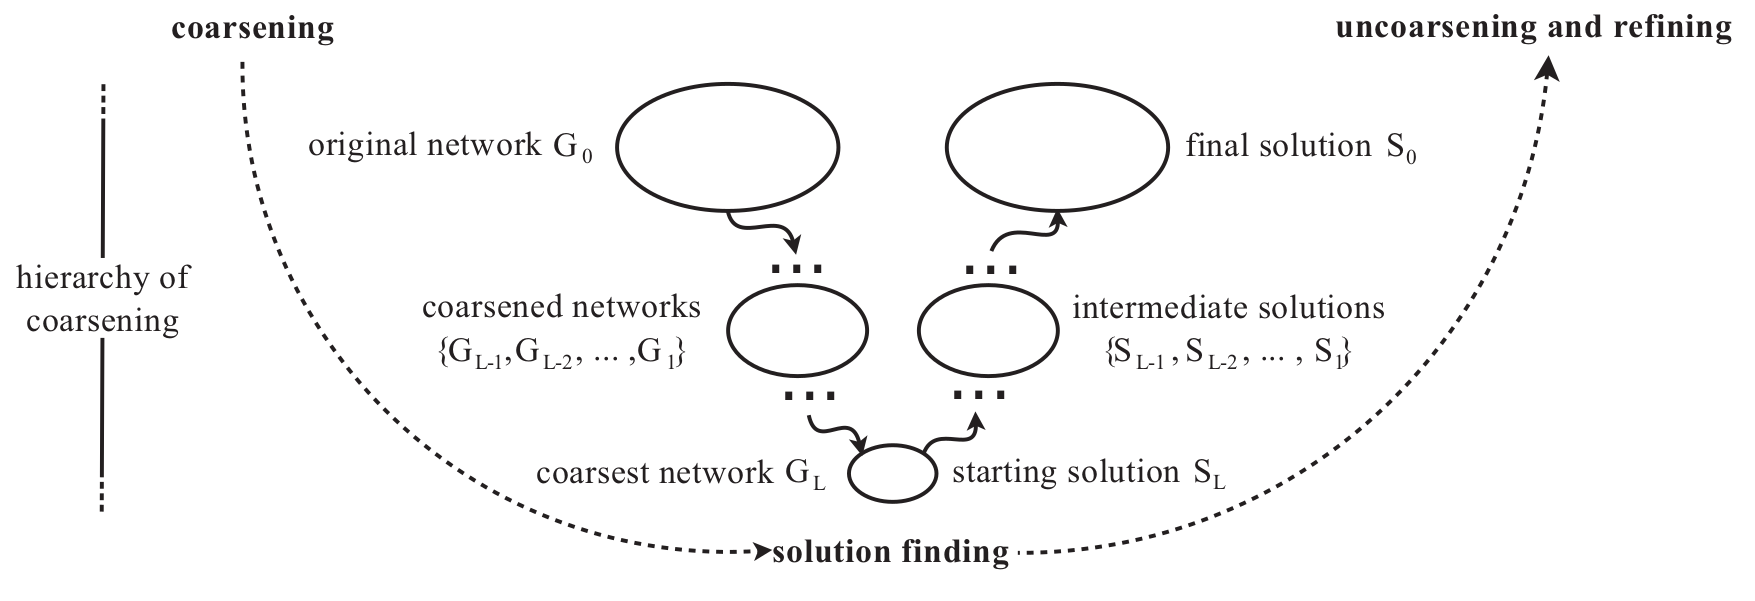
\includegraphics[width=\textwidth]{mlf}
  \caption{Phases of the multilevel optimization.
  A sequence of incrementally reduced networks is obtained in the coarsening phase.
  An initial solution found at the coarsest network, in the solution finding phase,
  and is projected back to the initial, uncoarsened, network, in the uncoarsening phase.
  Further details are given in Section~\ref{bac} and specificities related to these
  phases when applied to interactive data visualization are in Sections~\ref{net} and~\ref{nav}.
  }\label{mlf}
\end{figure}

The coarsening phase results in a sequence of networks $G_l$ from the initial network $G_0$,
on multiple levels of details.
The process is carried out by two algorithms: \emph{matching}, which decides which nodes to merge,
and \emph{contracting}, which achieves the reduced representation from the network and the matching.
In general, pairs of nodes are selected to be merged into supernodes, and
most often a matching $M$ consists in a set of non-adjacent links,
i.e. $\forall\; l_1, l_2 \in M, u \in l_1 \Rightarrow u \notin l_2$.
The heavy-edge matching, for example, is a matching that fits this canonical description
in attempting to maximize total matching weight, but the matching may not satisfy such restrictions.
Selecting clicks and other larger node sets to be merged into supernodes are possibilities
under development.
%%%
% citar alguem aqui?
For bipartite network, we use the algorithms provided by~\cite{alan2} in which two restrictions
are imposed to the matching:
\begin{itemize}
  \item A node may only match nodes on the same layer.
  \item A node may only match nodes that are reachable by two successive links
    (i.e. the closest possible nodes on the same layer).
\end{itemize}

The matching is followed by the contraction of the network into a coarser form.
Typically, the nodes matched are merged into a supernode
with the weight equal to the sum of the weight of nodes it contains,
and the links incident to such nodes are joined into superlinks among the supervertices,
also with total weight equal to the sum of the weights of the links merged.
The solution finding phase is usually reasoned about in terms of the computational cost, being much
alleviated in the reduced network.
The uncoarsening is usually performed through the complete hierarchy,
from the coarsest to the original network, with successive refinement of the solutions to
avoid local minima and improve solution quality.
These two phases are substantially different when the multilevel strategy is applied to visualization,
which motivated their separate exposition in the next subsection.

\subsection{Network visualization assisted by multilevel strategies}\label{net}
In applying the multilevel framework to visualization, adaptations are suitable to
the achievement of the visualization intended.
Such adaptations for our interactive visualization solution is as follows.
The target algorithm is the visual mapping of the network,
i.e. the solution finding phase is the visualization of the network by means of
the reduced representation.
The uncoarsening is performed only on demand through user requests
to visualize network supernodes in more detail,
thus avoiding unnecessary complexity and,
most importantly, avoiding to overload the visualization with information beyond the
cognitive convenience of the user and the computational power that the machine being used
is able to provide for real-time interactivity.

The interactivity is crucial for a number of reasons:
the specification of the coarsening algorithm;
the definition of the uncoarsening desired;
to enable the navigation of the network,
including the access to metadata and changes to the visualization achieved;
and for tuning the achieved visual mapping status, such as by resizing
and moving nodes.
The overall procedure is delineated in Algorithm~\ref{alg} and further
detailed in Sections~\ref{nav} and~\ref{sof}.


\SetKwData{Matching}{Matching$_b$}
\SetKwData{Contracting}{Contracting$_b$}
\SetKwData{map}{map\_to\_screen}
\SetKwData{trans}{transform\_visual\_mapping}
\SetKwInOut{Return}{Return}
\begin{algorithm}
  \KwIn{\\
  \quad bipartite network: $G$\\
  \quad maximum number of levels: $L \in [0,n] \subset \mathbb{Z}$\\
  \quad reduction factor for each layer: $rf_1, rf_2 \in (0,0.5] \subset \mathbb{R}$.\\
  \quad layers to be coarsened: $layers \in \{1,2\}$\\
  \quad user command given through the visual interface: $C$
  }
  \KwOut{\\
  \quad Visual mapping of the network: $V$}
  \BlankLine
  $i \leftarrow 1$\;
  \While{$i \le$ layers}{
    $l\leftarrow 1$\;
    \While{$l\leq L$}{
      $M \leftarrow$ \Matching{$G_l$, $i$, $rf_1$, $rf_2$}\;
      $G_{l+1} \leftarrow$ \Contracting{$G_l$, $M$}\;
      increment $l$\;
    }
      increment $i$\;
  }
  $V \leftarrow$ \map{$G_L$}\;
  \While{$C$ is not '$exit$'}{
    $C\leftarrow$ user command\;
    $V\leftarrow$ \trans{$V$, $C$}\;
  }
  \caption{An algorithmic description of the multilevel strategy adapted for the visualization of bipartite networks.
  The routines {\bf Matching$_b$} and {\bf Contracting$_b$} are any of the matching or contracting
  algorithms suited for bipartite networks, such as described in~\cite{alan2} which are the only ones
  currently available to the knowledge of the authors.
  The {\bf map\_to\_screen} routine is performed through the use of a network layout algorithm and
  then the rendering of the network to the screen.
  The visual mapping may then be transformed by the user by requesting uncoarsening of specific supernodes,
  or by other commands available to assist in the visualization,
  such as requesting metadata exposition, changes to the position of nodes, the color or transparency of nodes and links, zoom and pan,
  or any other operation defined in Section~\ref{sof}.}\label{alg}
\end{algorithm}

\subsection{The navigation pathway}\label{nav}
The abundance of information within large networks makes pertinent the
application of
the ``visual information-seeking mantra'', also known as Shneiderman's mantra:
\emph{overview first, zoom and filter, then details-on-demand}.
This mantra comprises a number of visual design guidelines,
such as the details-on-demand technique, and provides
a very acknowledged framework for designing information visualization applications.
Accordingly, our idealized exploration pathway starts with an overview,
achieved by the visual mapping of the coarsest representation of the network through
standard network layout algorithms for node-link diagrams.
The user may then zoom into specific regions of the network, and then request
details by a number of operations, most importantly:
\begin{itemize}
  \item reposition nodes, exposing linking patterns.
  \item request metadata, e.g. for a node, one may request to know the number of predecessors,
    the successor in a subsequent level, or the number of neighbors (i.e. the degree).
  \item request the visual mapping of network features, such as node size related to number of neighbors or the number of predecessors the node represents.
  \item request the uncoarsening of specific supernodes or any arbitrary group of supernodes.
\end{itemize}

Other operations are convenient to make the visual mapping adequate for the diverse settings possible:
network size, open supervertices, levels exposed, and topological features such as community structures.
These operations are detailed in Section~\ref{sof}.
The navigations pathway, already as achieved within the software we made available, is illustrated in Figure~\ref{fnav}.

\begin{figure}[!h]\centering
 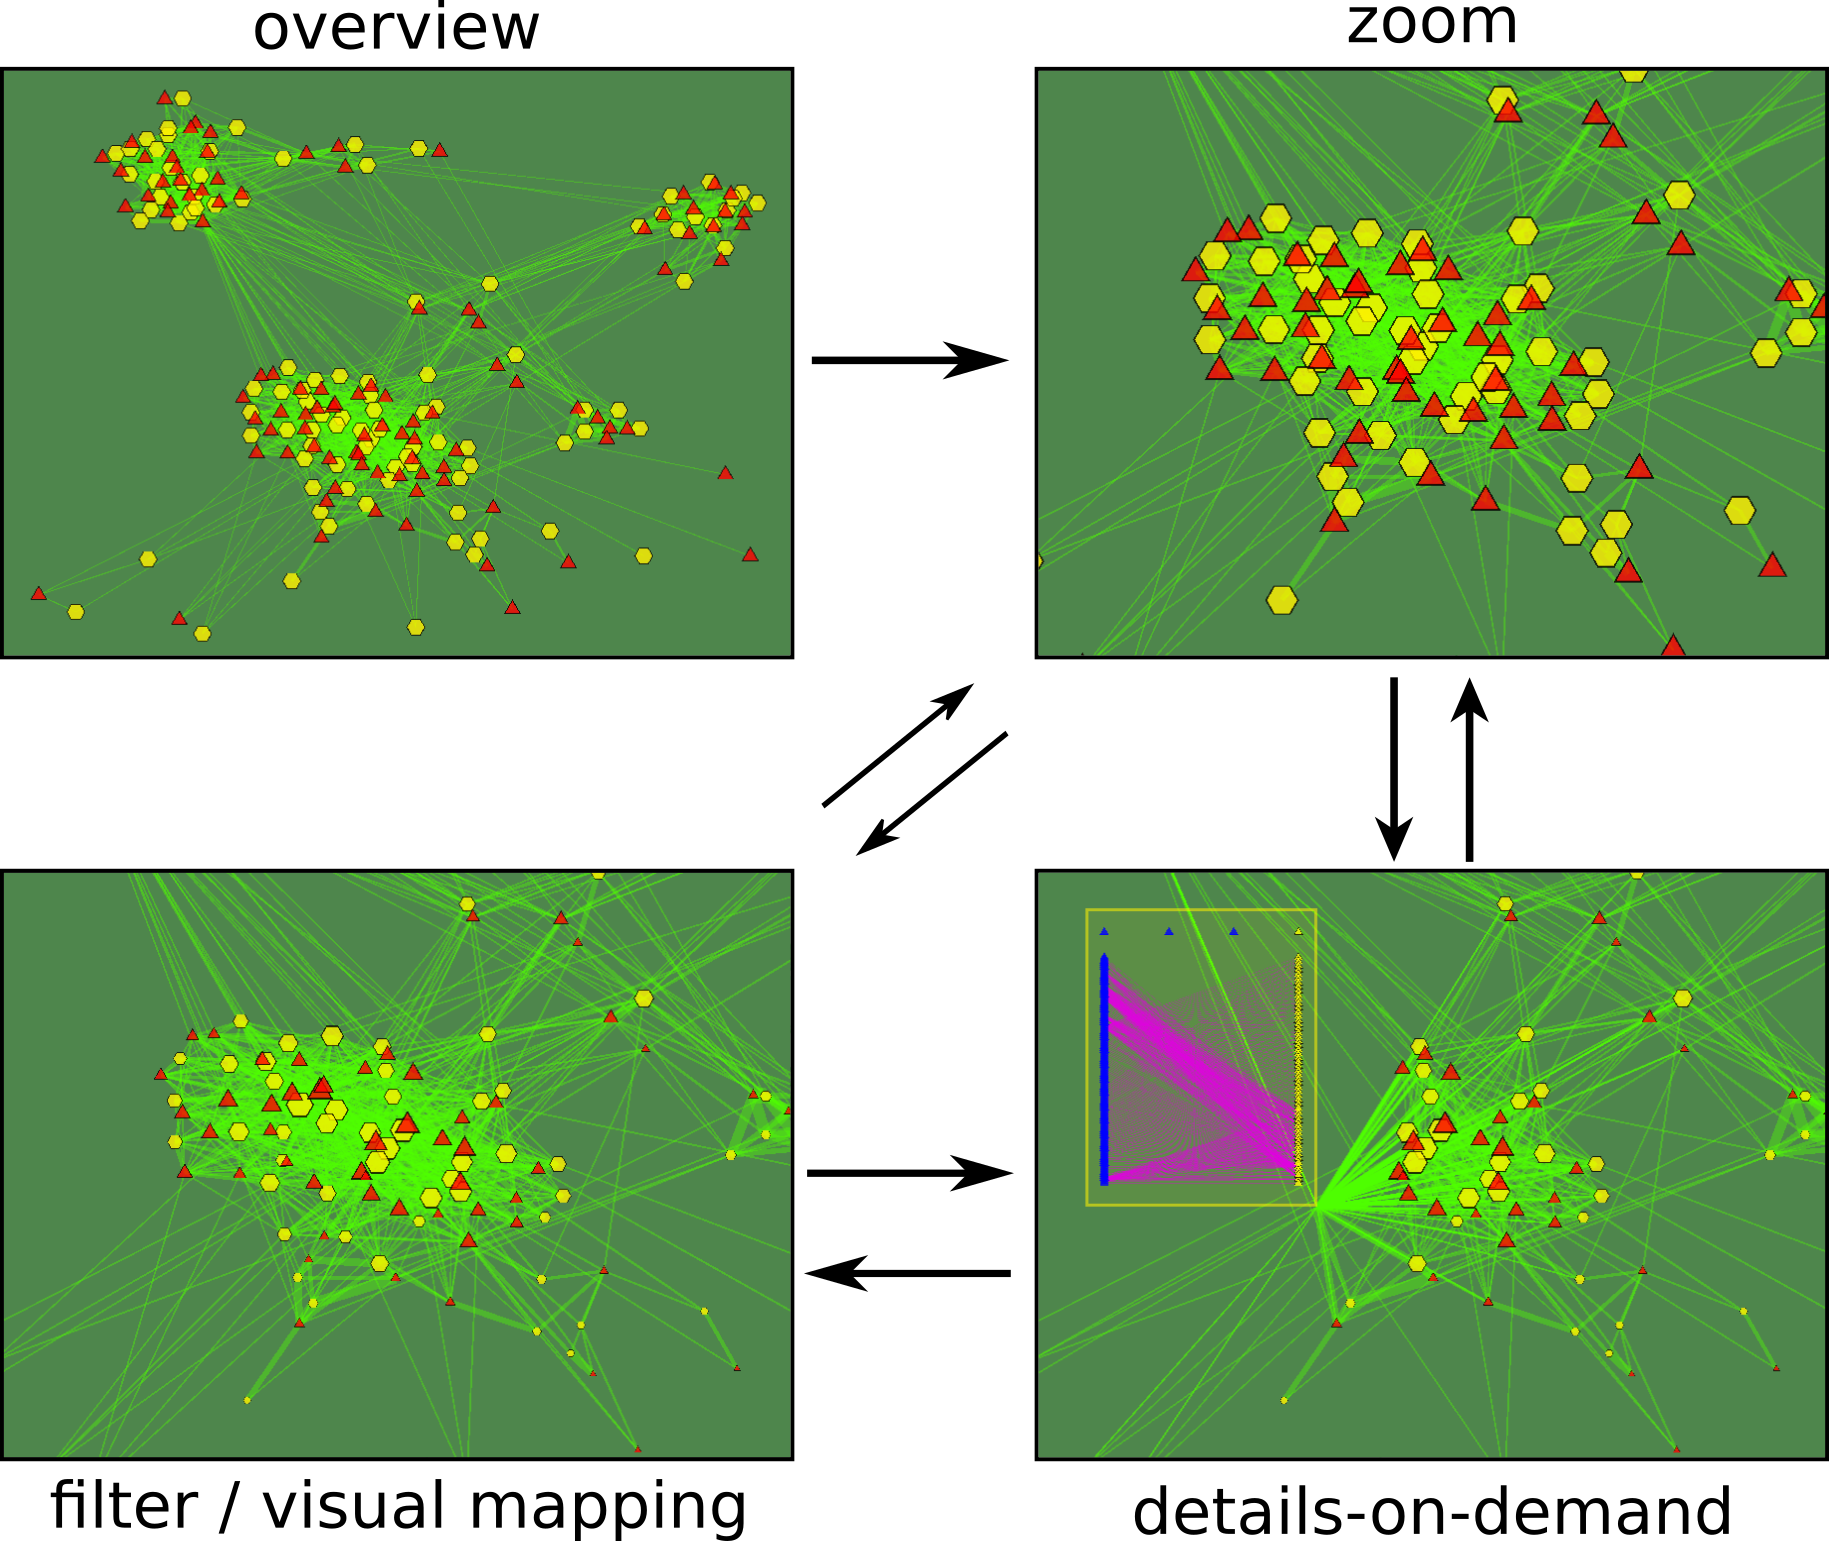
\includegraphics[width=0.8\textwidth]{fnav___}
  \caption{The navigation pathway of bipartite networks obtained through a multilevel strategy
  and auxiliary tools.
  Compliant with the Shneiderman's mantra, first and overview of the bipartite network is provided.
  Then the user may select an specific portion of the network to visualize in further detail,
  apply filters and visual mappings of topological features, and request details.
  These operations may be carried on in any order and any number of times the analyst understand convenient.
  }\label{fnav}
\end{figure}

\noindent 
\section{Software implementation}\label{sof}
% optimization of the computational capacity for large networks by
% means of Web GL, triangles for nodes and details on demand
We implemented the framework described in Section~\ref{des} using scientific,
database and web resources,
and made the final result available to the user within a web page
for use through simple mouse-driven actions
and requiring the installation of no software but a web browser such as Firefox or Google Chrome.
The final software was named MlBiNetVis (from Multilevel Bipartite Network Visualization)
and is exemplified in Figures~\ref{fpage0},~\ref{initial} and~\ref{secondPhase}.
Next subsections describe its functionalities and the technologies used.

\begin{figure}[!h]\centering
 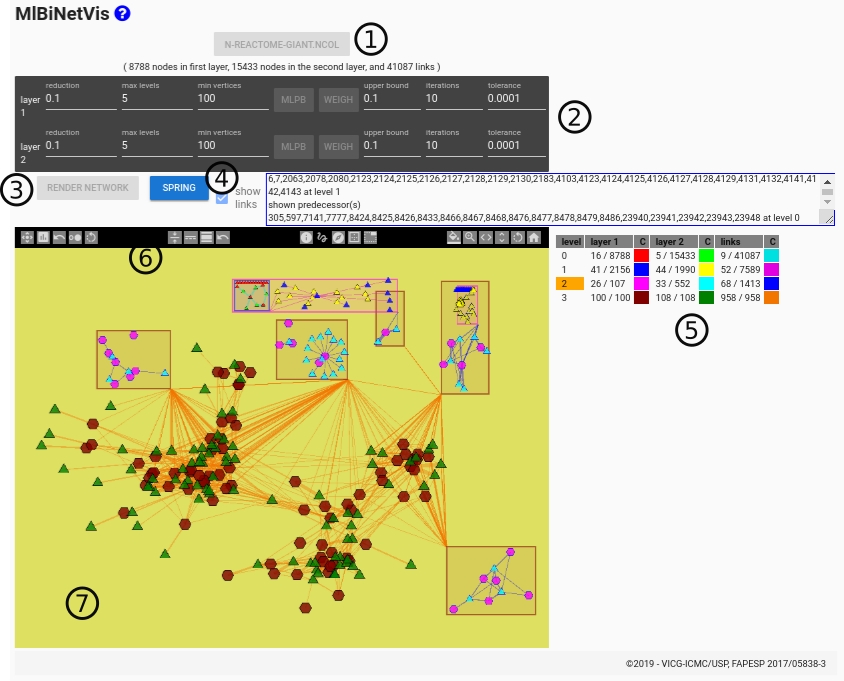
\includegraphics[width=\textwidth]{overall____}
  \caption{The MlBiNetVis interface. (1) is the dropdown menu for choosing the network to analyse or uploading new ones.
  The gray box in (2) contains widgets to select and parametrize the coarsening algorithm.
  (3) is the render button, which maps the network to the screen.
  In (4) are auxiliary widgets for selecting the  layout, show/hide of links, and for the interface to output information requested by the user or useful to assist navigation.
  In (5) is an interactive table which holds information about the levels and layers of the bipartite network and may be used to set the visualization on the canvas.
  In (6) is the toolbar that enables the navigation of the network and fine-tuning the visualization.
  In (7) is the canvas in which the network is drawn through node-link diagrams.
  Section~\ref{use} describes the use of these elements in further detail.
  }\label{fpage0}
\end{figure}

\subsection{The use of MlBiNetVis}\label{use}
% network upload, format.
% layouts available
% algorithms available for coarsening, and their parametrization
% initialization of the visualization: click on render
% tools available and their operation
In using MlBiNetVis,
the analyst first selects a network of interest to be explored.
One may also upload a network and then select it on the same drop-down menu.
The user may then wish to select one of the available network layout
algorithms and tune the coarsening to be performed, but default settings are reasonable
for the newcomer.
Upon request given by hitting the ``render network'' button,
the network is mapped to the screen.
Subsequent usage relies on manipulation of the visual mapping presented on the
canvas by means of actions
performed through managing the tools and related mouse operations.
These steps are illustrated in Figure~\ref{initial}.
\begin{figure}[!h]\centering
 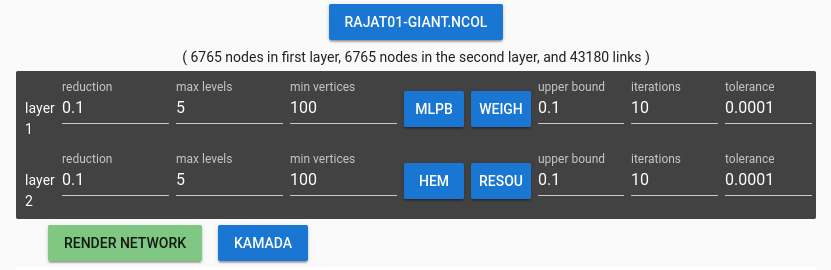
\includegraphics[width=\textwidth]{initial_}
  \caption{The elements in the initial step of the MlBiNetVis usage.
  The button at the top is for network upload and selection.
  In the gray box, the user chooses and sets the coarsening algorithm as detailed in Appendix~\ref{ap}.
  The blue button at the bottom is a drop-down menu where the user picks the node-link
  layout algorithm.
  The green button is for rendering the network to the canvas and initializing further widgets.
  By hitting the green button, all the elements in this image is made disabled, except for the layout
  button.
  Further information is given in Section~\ref{use}.
  }\label{initial}
\end{figure}

There are multiple levels of representation entailed by the multilevel strategy.
This makes pertinent that one and only of the available levels is explicitly selected
so that the transformations are performed on that level.
Thus, there is always a selected level in which the tools perform actions, such
as link coloring or opening supernodes to expose their predecessor nodes.
As can be inferred by the reader,
the number of nodes and links in each level which are visible are not fixed throughout the
navigation.
The selection of the level to which the transformations should apply, and the number
of visible and total nodes and links in each level, are exposed in the table to the right
of the canvas, as in Figure~\ref{secondPhase}.
In the same table, the user may change the color and shape of the nodes in each layer of
a level, the color of the links of a level, and toggle show/hide of the links is a level,
by left/right clicks on the corresponding colored cell.

\begin{figure}[!h]\centering
 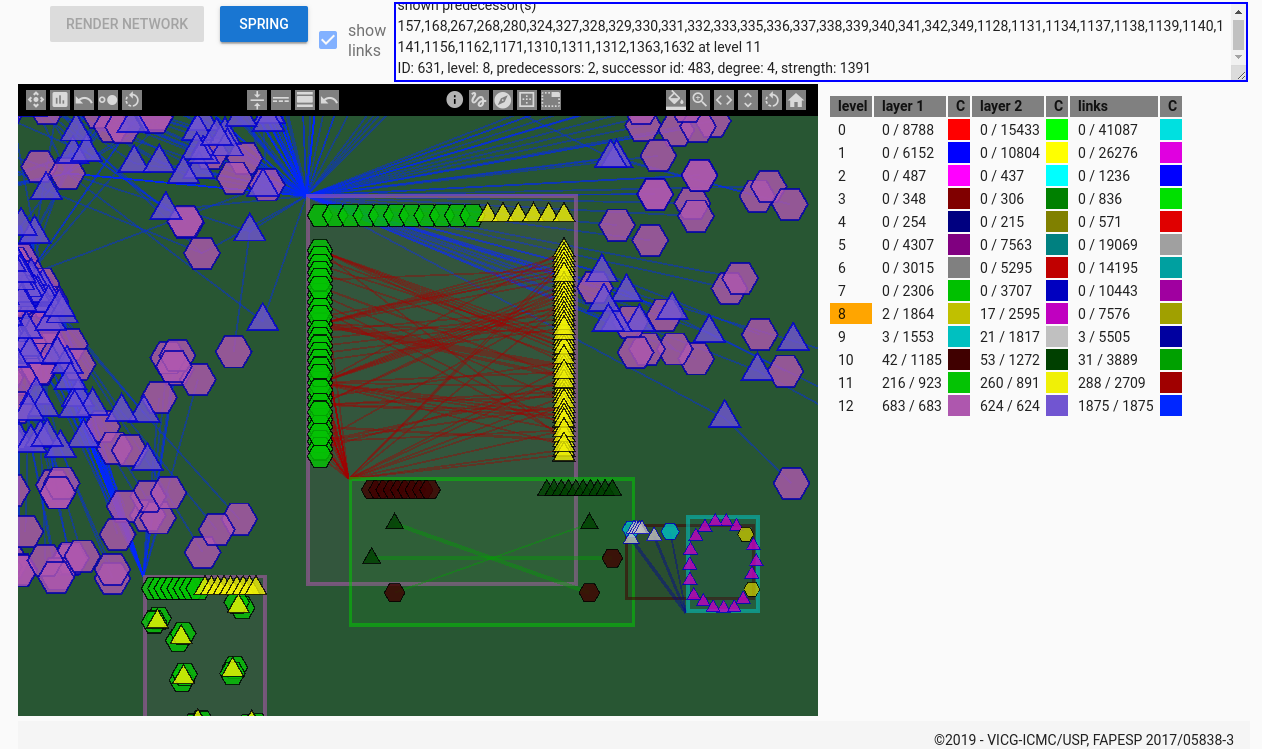
\includegraphics[width=\textwidth]{secondPhase}
  \caption{The elements in second step of the MlBiNetVis usage, dedicated to navigation on the network and transformation of the visualization.
  The user may change the layout used when supernodes are opened and the predecessors are then shown on the screen.
  Links may be shown or hided for all the levels by using the checkbox.
  The text area assists in the output of information requested or useful for navigation.
  The canvas holds the node-link representations of the levels, which are transformed using the tools in the toolbar and the table in the right-side.
  Such table also makes evident key information about the status of the visualization.
  Further information is given in Section~\ref{use}.
  }\label{secondPhase}
\end{figure}

The toolbar holds buttons for further actions to be performed and are divided in groups.
The first group is for changing how the nodes are visualized: size, proportionality to
the number of neighbors or predecessors, reset proportionality, transparency, and rotation.
The second group of buttons is for the links: thickness, transparency, proportionality to weight
using thickness or transparency, and reset proportionality.

The third group of buttons is more specific to the needs of the MlBiNetViz, and
are selected to make mouse operations entail special processes and transformations of the visualization.
The first button is selected for the interface to return core information from a clicked node:
id, level, number of predecessors of previous level, id of successor (if node is not on the last level),
number of neighbors (degree), sum of weight of links (strength).
Other information the analysts report necessity of are easily implemented, but currently only these informations
are returned to avoid unnecessarily flooding the text area.
The second tool button is selected to move nodes: specific nodes are individually moved if clicked and dragged;
a rectangular region is made available for moving all nodes therein if an empty region of the canvas
is clicked and the mouse cursor dragged before releasing the button.
The third tool button is selected for opening supernodes and exposing their predecessor nodes and links among them:
a region is defined by the user by clicking on an empty space on the canvas and dragging the mouse before releasing,
the supernodes therein are joined into a rectangular region that contains all of them,
and their predecessor nodes (which are on a finer level of detail) are drawn inside such rectangular region.
Open supernodes may be joined using the same tool, but it was found convenient to make available a
fourth button to assist in this task: if this tool is selected, one may join two open supernodes by
clicking on them in sequence.
The last tool button in this group is selected to perform three operations on open supernodes:
if an open supernode is clicked on and dragged, the rectangular shape is resized accordingly;
if there is no drag, i.e. the super node is clicked on and released, the links from it to the other
supernodes are attached to the next counterclockwise corner of its rectangular region.
When the open supernode is resized, the layout of its child nodes is optimized for the drawn region.
This is most useful when used in combination with the drag tool:
on the finer level of detail, the nodes are repositioned into a more compact disposition.
Then upon a (potentially minimal) supernode
resize, the child nodes are made to fit the whole rectangular area.
The last set of tools acts on the whole canvas:
changing the color of the background, zoom, left-right/up-down pan,
rotation of the entire network,
and toggling between current zoom and pan status and the initial setting.
The toolbar is contextualized in Figure~\ref{secondPhase}.

There are many subtleties on the orchestrated use of these tools.
As a facilitated means to convey the navigation possibilities and
procedures available, the user is invited to watch a demo video in~\cite{yvideo},
and use the MlBiNetVis interface through the instance we made available~\cite{mbnvpage}.
The more seasoned software developer may browse the code, upload a local instance
of the software, and make changes to its source code~\cite{mbnvcode}.

\subsection{Software technologies employed within mlvis}
% coarsening algorithms
% flask for server, feather for auxiliary server
% mongodb filesystem for data
% Nuxt/Vue.js for the frontend with heavy use of PIXI.js
Most important parts of MlBiNetViz are written in a combination of JavaScript and Python:
Vue.js (set up by Nuxt.js) is used to assist in the client (frontend),
the server (backend) is a Flask Python server, used to perform
specialized or heavy calculations.
There is a secondary server, a FeatherJS, used to facilitate contact with the database
and real-time multi-user interaction.
The data is stored in a MongoDB database and ordinarily in the file system,
while the multi-user interaction was deactivated for now to avoid unnecessary complexity.
The coarsening algorithms for bipartite networks are available in~\cite{bialgs}
and are used by the Flask server.
The fast WebGL 2D rendering on the canvas is performed using Pixi.js.

The rasterization of images is usually performed though triangles.
Accordingly, in order to comply with the goal of enabling the visualization of large bipartite networks,
the rendered network on the canvas contains only triangles (one for each of the nodes) and straight lines (for the links).
The user may wish to further alleviate the computational cost by not showing the links.
To emphasize the bipartite structure of the network, and for making the visualization more aesthetically
compelling, the user may change the shape of the nodes in one (or both) of the layers to hexagons instead of triangles.
Using these features, and within the technologies described, we have visualized networks
with tens of thousands of nodes without perceiving any lag in the interactive navigation and transformations,
with links shown,
even using ordinary machines (e.g. with 8GB RAM DDR3, an i7 processor of the first generations, and a 1GB GPU).

This is a very brief account of the styles and software resources used to implement
MlBiNetVis. The interested reader is welcome to browse the software code and documentation
and contact the authors~\cite{mbnvcode}.

% \section{Results and discussion}\label{res}
%%%
% consistent use of overview first, details on demand
% a first contribution on ML vis. of bipartite networks
% simple interactivity strategies
% enhancements of the navigation through the use of being-developed coarsening algorithms
% the use of the interface for guiding coarsening (through markers)
% the use of the interface to analyse coarsening results

% technologies used: maybe simpler if using meteor.js
% and simpler to achieve multiuser interactivity

\section{Conclusions and further work}\label{con}
%%%
% extension to multipartite (or heterogeneous) networks.
We have described and made available the first visualization interface for bipartite networks
assisted by multilevel strategies.
The resulting conceptual organization is very consistent with the Shneiderman's mantra,
as exemplified the by the implemented software.
The interface developed is efficiently managed through simple interactive operations,
and very efficient in visualization large networks due to the use of multilevel strategies,
the software technologies employed, and the computationally inexpensive design decisions regarding
the rendering of the node-link diagrams.
In summary, this work is a proof-of-concept in that it establishes as feasible the use
of multilevel strategies for the visualization of large bipartite networks.

In further steps, the navigation may be enhanced by the acute use of in-development coarsening algorithms.
The visualization pathway is being envisioned as capable to assist the development of novel
multilevel strategies, which should be verified.
Also, there are multilevel strategies that involve the selection of nodes as pivots
to guide the coarsening procedure, a process to which there is no visual interface,
and to which MlBiNetVis should be adapted.
Also, the interface is envisioned to assist the analysis of coarsening results. As in the current version of MlBiNetVis,
the analyst is able to scrutinize linking patterns and overall network structure though the node-link diagram,
and requesting information, but this should be enhanced by the display of histograms and global measures of each level.
On the analysis of the networked structures, the navigation involving metadata, such as from genes and proteins, or as
documents and authors, should result in a visual analytics interface for interactive knowledge discovery.
Finally, bipartite networks are naturally extended to heterogeneous (or multipartite) networks,
and thus all the content of this article, and should require further research and development for the achievement
of concrete derivatives.

\appendix

\section{Choice and fine-tuning of the coarsening algorithm}\label{ap}
The elements in Figure~\ref{initial}.

\bibliographystyle{splncs04}
\bibliography{biblio}
%
% \begin{thebibliography}{8}
% \bibitem{ref_article1}
% Author, F.: Article title. Journal \textbf{2}(5), 99--110 (2016)
% 
% \bibitem{ref_lncs1}
% Author, F., Author, S.: Title of a proceedings paper. In: Editor,
% F., Editor, S. (eds.) CONFERENCE 2016, LNCS, vol. 9999, pp. 1--13.
% Springer, Heidelberg (2016). \doi{10.10007/1234567890}
% 
% \bibitem{ref_book1}
% Author, F., Author, S., Author, T.: Book title. 2nd edn. Publisher,
% Location (1999)
% 
% \bibitem{ref_proc1}
% Author, A.-B.: Contribution title. In: 9th International Proceedings
% on Proceedings, pp. 1--2. Publisher, Location (2010)
% 
% \bibitem{ref_url1}
% LNCS Homepage, \url{http://www.springer.com/lncs}. Last accessed 4
% Oct 2017
% \end{thebibliography}
\end{document}
